\documentclass{l4dc2027}
% Paper B — LONG FORMAT v1 (the first full draft, ~4 700 words of text; compiles to ~16 pages). Kept at the user's request
% (2026-11-01) as a reference for later venues. The submission version is ../main.tex.
\usepackage{times}
\usepackage{booktabs}
\usepackage{siunitx}

\makeatletter
\@ifundefined{proposition}{\newtheorem{proposition}{Proposition}}{}
\@ifundefined{remark}{\newtheorem{remark}{Remark}}{}
\@ifundefined{definition}{\newtheorem{definition}{Definition}}{}
\makeatother
\newcommand{\vmax}{v_{\max}}
\newcommand{\wmax}{\omega_{\max}}
\newcommand{\adm}{\mathcal{A}}
\graphicspath{{../../figures/}}

\title[Safe and Stuck]{The Guarantee Holds and the Task Fails: Absorbing Stalls of Learned Policies under CBF Filters}

\author{%
 \Name{Mohammad Shoaib} \Email{[to confirm]}\\
 \addr NSU Intelligent Robotics Lab, North South University, Dhaka, Bangladesh
 \AND
 \Name{Shahnewaz Siddique} \Email{shahnewaz.siddique@northsouth.edu}\\
 \addr Department of Electrical and Computer Engineering, North South University, Dhaka, Bangladesh%
}

\begin{document}

\maketitle

\begin{abstract}%
A safety filter that projects a learned policy's command onto an admissible set guarantees that the safe set is forward invariant. It guarantees nothing about progress. We show that a control barrier function (CBF) filter placed in front of a memoryless learned pursuer creates a closed-loop fixed point at which the guarantee holds, violations are zero, and the task fails silently: the filter zeroes the command, the body stops, the observation freezes, and the policy re-emits the same command for the rest of the episode. We state the fixed point as the known normal-cone condition for CBF-QP deadlock applied to a learned nominal, add three learning-side refinements, and measure it: every stalled state lies on the filter's exact tier, 98\% are traps at the current heading, and none is a trap of the position. We measure why learning does not remove it: the reward for escaping arrives 629 steps later and is worth 0.009 at $\gamma = 0.99$. Across seven pre-registered rounds, every learning-side remedy improves the task and none removes the failure, a stall penalty makes it worse, and a one-counter recovery that offers filtered forward and rotation candidates after $N$ immobile steps clears the deadlock on all three policy families (0.19--0.30 to 0.000), raises capture on nine of nine seeds with zero violations, is insensitive to $N$ over 5--80 steps, and composes onto a second filter. Three dissociations show liveness metrics improving while the task collapses.%
\end{abstract}

\begin{keywords}%
safety filters; control barrier functions; shielding; safe reinforcement learning; deadlock; liveness; pursuit--evasion%
\end{keywords}

\section{Introduction}\label{sec:intro}

Safety filters wrap a learned policy with a guarantee. A control barrier function (CBF) filter, a shield, or a predictive filter takes the policy's command, tests it against a safe set, and replaces it with the nearest admissible command when the test fails \citep{hsu2024safetyfilter,ames2019cbf,alshiekh2018shielding,cheng2019endtoend}. The guarantee is forward invariance of the safe set. It says nothing about the task the policy was trained for, and the two can come apart in a way that no violation count reveals.

Figure~\ref{fig:frozen} shows the failure in one archived episode. A pursuer trained with proximal policy optimisation, deployed behind a CBF filter, drives toward an obstacle that stands between it and the evader. The filter zeroes its forward command. The body stops, the observation stops changing, and the memoryless policy emits the same full-speed command at every one of the next 1\,106 steps, with a standard deviation of 0.000 across them, while the executed speed stays at zero. The episode ends in a timeout. The same episode under the recovery of Section~\ref{sec:formal}, same seed and same evader, ends in a capture at step 262. The violation count is zero in both.

This is not the multi-robot deadlock of the CBF literature, although it shares its algebra. There, deadlock is a force equilibrium between agents whose constraint normals cancel the nominal \citep{grover2020symmetry,grover2021deadlock,grover2023before}; here one agent stands against static geometry. The nearest prior objects are the undesired equilibria that CBF quadratic programs introduce into the closed loop of a fixed nominal controller \citep{reis2021cbfqp,tan2024undesired}. Our object is what happens when the nominal is a policy that was trained through the filter and that sees the world only through an observation the stall has frozen. The trap is in observation space, not in the force balance, and that is why learning does not escape it.

\paragraph{Contributions.} (C1)~A characterisation of filter-induced stalls for learned memoryless policies, with the distinction between a trap of the position and a trap of the policy--filter pair at a heading, measured on 262 stalled states (Proposition~\ref{prop:stall}, round~B1). (C2)~The mechanism that defeats learning: a frozen input and a reward for escape that arrives about 630 steps later, measured on 383 stall entries (Section~\ref{sec:formal}, round~S15). (C3)~A pre-registered comparison in which every learning-side remedy improves the task and none removes the failure, a stall penalty backfires, and a one-counter forward-offering recovery removes the failure without touching the guarantee, across three policy families, a parameter sweep, a perturbation baseline, and a second filter class (Proposition~\ref{prop:recovery}, rounds~S16, S17, B2--B4). (C4)~Three pre-registered dissociations between filter-adjacent liveness metrics and the task (rounds~S16, S18, S19), which make a measurement recommendation for papers that evaluate filtered learned policies.

Every number in Sections~\ref{sec:experiments} and~\ref{sec:dissociations} comes from a pre-registered round with a frozen commit, paired seeds, and a record that was written before the hypothesis was read. Section~\ref{sec:related} places C1 against the deadlock literature and C3 against the conservativeness fixes proposed at this venue.

\section{Related work}\label{sec:related}

\paragraph{Deadlock and undesired equilibria of CBF-QP controllers.} \citet{grover2020symmetry,grover2021deadlock,grover2023before} characterise multi-robot deadlock under CBF quadratic programs through the Karush--Kuhn--Tucker conditions: the projected command is zero exactly when the nominal lies in the conic hull of the active constraint normals, a force equilibrium, and the deadlock set has measure zero. \citet{reis2021cbfqp} showed that CLF--CBF quadratic programs create spurious asymptotically stable equilibria on the boundary of the unsafe set even for a single agent and one convex obstacle. \citet{tan2024undesired} characterised all closed-loop equilibria of such programs and modified the program to remove the undesired ones while keeping forward invariance; \citet{reis2026stability} and \citet{reis2025unified} extended the stability analysis, the latter stating explicitly that safety is guaranteed and liveness is not. These works fix the filter. We keep the filter and its guarantee untouched, show that a learned nominal makes the equilibrium absorbing in observation space, and remove it with a stateful shield outside the filter.

\paragraph{Shield conservativeness.} \citet{kim2025realizable} require that a continuous-space shield always has a safe action to offer, including stateful requirements such as loop avoidance, and note that the shield alone leads to overly conservative behaviour; the remedy is on the specification side. \citet{dawood2025dynamic} let a learned supervisor adapt the weights of an MPC shield to reduce conservativeness. \citet{wang2025neurosymbolic} resolve multi-robot deadlocks after they occur with a guarantee of no persistent deadlock, and \citet{lee2025merrygoround} prevent them in decentralised teams. \citet{arnstrom2025stealthy} study the adversarial deactivation of filters. Our remedy is the minimal stateful addition, a single counter, evaluated on learned policies in an adversarial game; Proposition~\ref{prop:stall} predicts the oscillations and timeouts these papers report for any filter that executes the nearest admissible command.

\paragraph{Learning through the filter.} \citet{oh2026provably} show that a filter-unaware policy chatters against the filter and that treating the filter as part of the Markov decision process and training through it is optimal when the filter is permissive enough. \citet{wu2026competence} train through a filter to obtain minimally exploitable policies in a game. \citet{georgescu2026gr1} repair a GR(1) shield's specification online so that liveness stays achievable when the shield's assumptions fail, and \citet{nakamura2025latent} report that switching filters hurt task completion. \citet{pizarro2025filtering} penalise the magnitude of the filter's correction during training and find that it improves return and reduces chattering on a quadrotor tracking task. We measure the case in which training through the filter still fails: at the stall the filter is not permissive, and the signal that would teach the escape is discounted away. The remedy we give needs no retraining.

\paragraph{Metrics.} We found no prior work that separates filter-adjacent liveness metrics (immobility, deadlock episodes, intervention rate) from task success under pre-registration. Section~\ref{sec:dissociations} gives three instances in which they move in opposite directions.

\section{Setting and definitions}\label{sec:setting}

\paragraph{Game.} A unicycle pursuer ($v \le \SI{1}{m/s}$, $|\omega| \le \SI{2.84}{rad/s}$, $\Delta t = \SI{0.05}{s}$) hunts an evader in a $10 \times \SI{10}{m}$ arena with two circular obstacles. The pursuer senses within a $90^\circ$ field of view of range \SI{8}{m}; capture is contact within \SI{0.30}{m}; an episode lasts 1\,200 steps. The evaders are a greedy flee policy, an obstacle-hugging policy, and a learned attacker (ATK4-45) with full state that was trained to stall filtered pursuers. The pursuers are structured search policies: a PPO head that chooses a search action held for 10 steps when the evader is out of view, and a fixed intercept law when the evader is visible. Both branches are memoryless.

\paragraph{Filter.} The base filter is a discrete-time CBF projection. A candidate command is admissible if the exact one-step barrier condition holds on the true Euler successor state; among admissible candidates the filter executes the one nearest to the nominal in the weighted norm $w_v(\Delta v)^2 + w_\omega(\Delta\omega)^2$ with $w_v = 150$, $w_\omega = 1$, with barrier rate $\gamma_{\mathrm{cbf}} = 0.2$ and a virtual control point \SI{0.1}{m} ahead of the axle. The filter has three tiers (exact, relaxed, backup); every stalled state in this paper lies on the exact tier (Section~\ref{sec:phenomenon}). The second filter of Section~\ref{sec:second} is a sampling lookahead through the simulator with horizon 4 and the same interface. A violation is the simulator's contact flag; H-SAFE denotes the pre-registered requirement of zero contact steps in every filtered cell.

\paragraph{Definitions.} A step is \emph{immobile} if the executed speed is at most $0.05\,\vmax$; \emph{stalled} if immobile while the nominal speed is at least $0.5\,\vmax$; a \emph{self-stop} if immobile and not stalled. A \emph{stall run} is a maximal sequence of stalled steps; a \emph{deadlock episode} contains a stall run of at least $K = 40$ steps (\SI{2}{s}). A state is a \emph{filter trap at heading} if no admissible command at the current pose has executed speed above $0.05\,\vmax$; a \emph{position trap} if this holds at every heading at that position; a \emph{pair trap} if it is a trap at heading and not a position trap. An \emph{escape} is a displacement of \SI{0.10}{m} from the stalled pose. An \emph{engagement} is a cluster of recovery firings separated by fewer than five steps; a \emph{cycle} is an engagement that ends in a stall within 40 steps of the previous one. Admissibility is always the exact one-step test; where we say the filter returns a command unchanged we mean the exact tier accepted it.

\paragraph{Policies and rounds.} Table~\ref{tab:rounds} lists the rounds. The BASE, OBS, GAM and OBSGAM families (three seeds each) are trained from scratch for 5\,M steps behind the filter; OBS adds the filter's admissible-turn features to the observation, GAM raises the discount to 0.999, OBSGAM does both. STR14 and RC19 are 10\,M-step policies from the rounds in which the failure was first seen; RC19 observes the filter's state. All policies are frozen before any round that evaluates them.

\begin{table}[t]
\centering\footnotesize
\caption{Pre-registered rounds. Each round has a frozen commit, a specification with hypotheses and bars fixed before any number, paired seeds on a fresh seed stream, and a record under version control. H-SAFE held (zero contact steps) in every filtered cell of every round.}
\label{tab:rounds}
\begin{tabular}{@{}l p{5.6cm} p{4.5cm} p{2.5cm} r@{}}
\toprule
Round & Measures & Policies & Opponents & $N$ / cell \\
\midrule
S4, S5 & filter cost; first remedies & STR14; RA, RB, RC & six & 500 paired \\
S15 & mechanism (772 stall entries) & FT-B-41, RC19 & ATK4-45, Greedy & 200 \\
S16 & five learned remedies; rotation recovery & BASE, PEN, MEM, OBS, GAM, REC & ATK4-45, HUG7, Greedy & 500 paired \\
S17 & forward-offering recovery, seven families & BASE, OBS, GAM, OBSGAM, RECF & ATK4-45, HUG7, Greedy & 500 paired \\
S18 & correction-magnitude penalty, 18 arms & BASE, DVARY, SPARSE, DRARE & Greedy & 500 \\
S19 & law pins removed (planner law) & LINE, PLAN & Greedy, HUG, ATK4-45 & 500 paired \\
B1 & stall geometry; dwell (det.\ / stoch.) & BASE-60/61/62, RC19 & ATK4-45 & 100 \\
B2--B4 & $N$ sweep; baseline; second filter (86 cells) & BASE-60/61/62, STR14, RC19 & Greedy, ATK4-45 & 500 paired \\
\bottomrule
\end{tabular}
\end{table}

\section{Why a filtered memoryless policy stops}\label{sec:formal}

Let $s$ be the pursuer's state, $o(s)$ its observation, $u_\pi = \pi(o(s))$ the nominal command, and $\adm(s) \subset [0,\vmax] \times [-\wmax,\wmax]$ the set of commands that pass the exact one-step barrier test at $s$. On the exact tier the filter executes $P_{\adm(s)}(u_\pi)$, the projection of the nominal onto $\adm(s)$ in the weighted norm. The admissible set is the intersection of the command box with the half-spaces of the linearised barrier rows, hence convex, so the projection is unique.

\begin{proposition}[Stall characterisation]\label{prop:stall}
On the exact tier the executed speed is zero if and only if $u_\pi$ lies in the weighted normal cone of $\adm(s)$ at the zero-speed face, equivalently $u_\pi = \sum_{j \in J(s)} \mu_j a_j$ with $\mu_j \ge 0$ over the active barrier normals $a_j$. If moreover $o(s)$ is constant along the stall, the closed loop is at a fixed point and the stall is absorbing for the rest of the episode.
\end{proposition}

\begin{proof}[Proof sketch]
Projection onto a closed convex set in a Hilbert norm returns the point $u^\star$ with $\langle u_\pi - u^\star, u - u^\star\rangle_W \le 0$ for all admissible $u$; at $u^\star$ on the zero-speed face this is the normal-cone condition, and stationarity of the Lagrangian gives the conic combination of active normals, which is the force-equilibrium condition of \citet{grover2023before} written for one agent and static constraints. If $o(s)$ does not change, $\pi$ returns the same $u_\pi$, the projection returns the same zero-speed command, and $s$ does not change.
\end{proof}

The characterisation is known; what the learned setting adds are four refinements, which the rounds of Section~\ref{sec:experiments} measure. (R1)~\emph{Position trap versus pair trap.} A stall at pose $(p,\theta)$ can be a trap at heading $\theta$ while some other heading at $p$ admits forward motion. A rotation in place changes $\theta$ and not $p$, so the pose is not a fixed point of the state, only of the position. What is trapped is the pair (policy, filter): the policy asks for the blocked direction, and the filter admits only commands the policy never asks for. (R2)~\emph{Eventual constancy.} The observation is a function of the pose, the opponent's visibility, and bounded filter features whose stall-run counter saturates at 80 steps. Whenever the opponent is out of view, the input is therefore constant after at most 80 stalled steps, and the loop is at a fixed point of the observation from then on. This is why filter-state features alone (the OBS family and RC19) recover part of the task and not the failure: they move the fixed point, they do not remove it. (R3)~\emph{Exploration.} For a Gaussian head one might expect the stall to end once a sampled action displaces the body, with a geometric dwell. Round B1 does not support a dwell law, for a reason the game makes plain: the long stalls belong to the intercept law, which samples nothing, and where the head is in control the evader's motion ends the stall sooner than sampling would (Section~\ref{sec:phenomenon}). What survives is the weaker statement that the deadlock rate under stochastic sampling is no lower than under deterministic actions. (R4)~\emph{Two kinds of zero.} The nominal may itself be zero. A policy that has learned not to ask reaches the same fixed point as one whose request is blocked; Section~\ref{sec:dissociations} shows a penalty teaching exactly this.

\begin{remark}[Why learning does not remove it]\label{rem:discount}
Let $A_0$ be the undiscounted capture advantage of escaping a stall and $T$ the delay from the escape to the capture. By (R2) the escape's advantage attaches to one shared input vector, and under the training discount it is at most $\gamma^{T} A_0$. Round~S15 measured $A_0 = 0.257$ and $T \approx 629$ steps, which gives $0.0005$ at $\gamma = 0.99$, and a measured discounted advantage of $0.0092$; at $\gamma = 0.999$ the bound is $0.137$. This is an upper bound on a learning signal, not a proof that learning must fail; the GAM family ($\gamma = 0.999$) is the test, and it raises the task and does not clear the deadlock.
\end{remark}

\paragraph{The recovery.} After $N$ consecutive immobile steps, the shield filters the candidates $(\vmax,0)$, $(\tfrac12\vmax,0)$, the nominal, and $(0,\pm\wmax)$ in that order and executes the first whose filtered speed exceeds $0.05\,\vmax$; if none moves, it executes the larger admissible rotation. The counter resets on any mobile step.

\begin{proposition}[Recovery]\label{prop:recovery}
(a)~Every command the recovery executes is an output of the base filter on the current state, so the forward-invariance guarantee is exactly the base filter's; no assumption is added. (b)~If the stalled position is not a position trap, some heading admits forward motion; the admissible rotation reaches it within $T_{\mathrm{turn}} = 45$ steps at $\wmax$, after which the forward candidate passes, so the body typically leaves the position within $N + T_{\mathrm{turn}}$ steps. (c)~Nothing in (a)--(b) excludes a stall--recover--stall cycle; it is measured, not bounded.
\end{proposition}

Part (b) is stated with ``typically'' because round B2 found that 97.8\% of 10\,475 triggers meet the bound and the tail is reported, not explained (Section~\ref{sec:remedies}). Any filter that executes the nearest admissible command, including the closest-safe-action shield of \citet{kim2025realizable}, satisfies the hypothesis of Proposition~\ref{prop:stall}; the recovery is the minimal state, one counter, that breaks (R2) without changing $\adm(s)$.

\section{Experiments}\label{sec:experiments}

\subsection{Protocol}\label{sec:protocol}

Each round was specified before any number was produced: hypotheses, bars, the verdict rule for each, and the sentence to be written if a hypothesis failed. The code was frozen at a commit, cells were evaluated on fresh seed streams with the same seeds across arms, and paired differences were tested with the exact two-sided binomial test on discordant pairs at $p < 0.05$. Construct gates refuse to produce a summary: a round that shares cells with an earlier round must reproduce the earlier records bit for bit, and the animated episodes of designated cells must be watched before the summary runs. H-SAFE requires zero contact steps in every filtered cell. A stop rule forbids re-running or re-cutting a cell after its number exists. Every verdict in this paper is the registered one, including the failures.

\subsection{Phenomenon and mechanism}\label{sec:phenomenon}

\begin{figure}[t]
\centering
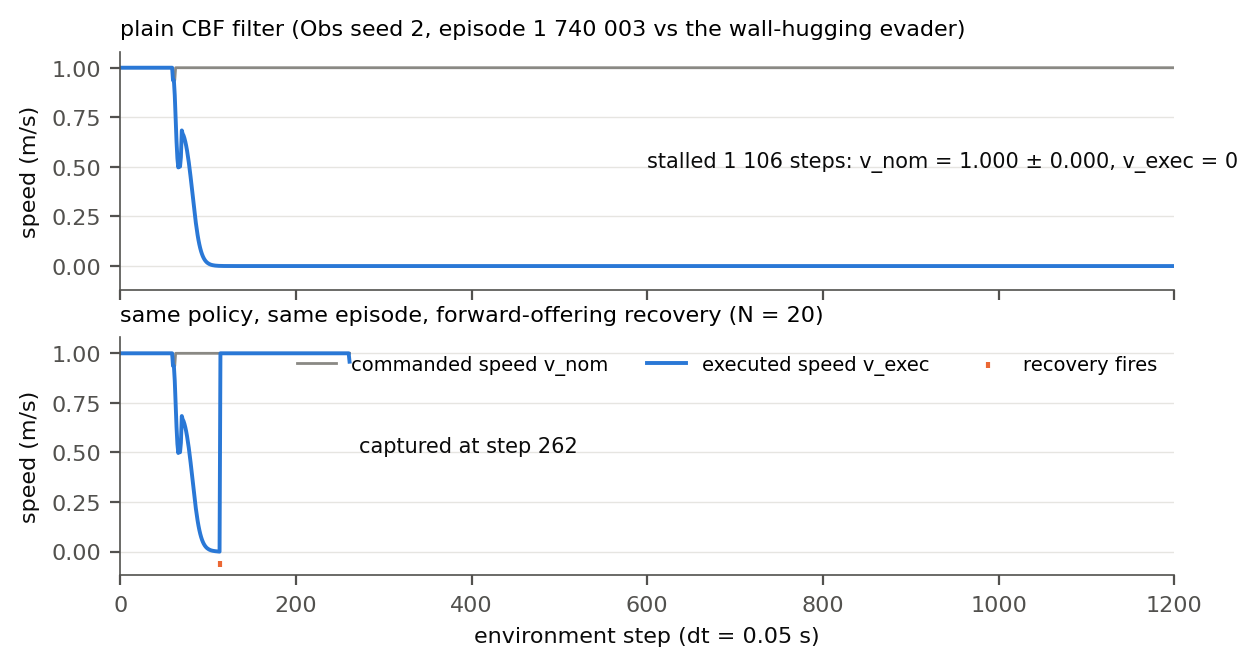
\includegraphics[width=\linewidth]{F1_frozen_input}
\caption{Frozen input. Nominal speed, executed speed and nominal turn rate over one archived episode of an OBS-family policy against the obstacle-hugging evader under the plain filter (round S17), and the same seed under the recovery. The bare episode ends in a timeout; the recovered one ends in a capture after a single firing.}
\label{fig:frozen}
\end{figure}

\begin{figure}[t]
\centering
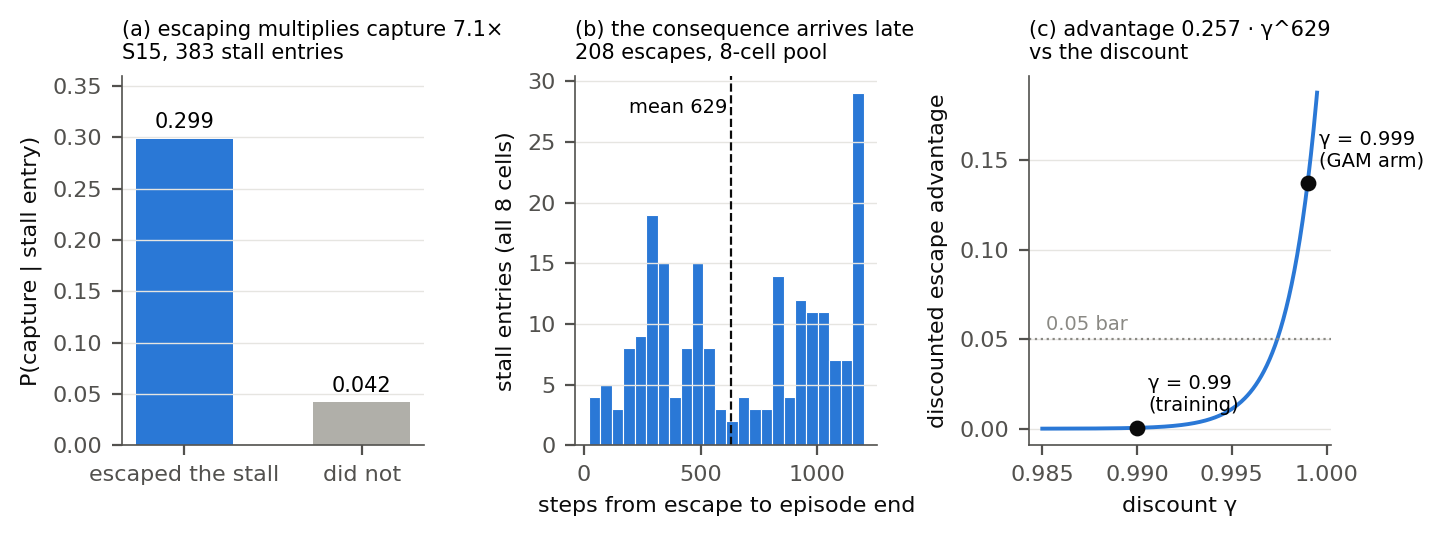
\includegraphics[width=\linewidth]{F2_mechanism}
\caption{Mechanism (round S15). (a)~Capture rate after a stall is escaped versus after it is not. (b)~Distribution of the delay from the escape to the capture. (c)~The discounted advantage bound $\gamma^T A_0$ as a function of $\gamma$, with the training values marked.}
\label{fig:mechanism}
\end{figure}

The filter's cost is large before any remedy. In round S4 the learned pursuer STR14 captured the greedy evader in 0.728 of 500 paired episodes without the filter and 0.396 with it ($p = 3\times10^{-44}$), a loss on five of six opponents and 2.5 times the loss the scripted teacher suffered under the same filter. In the filtered episodes 0.540 were deadlock episodes. Round S5 then showed that a stall penalty alone recovers nothing (0.426, 0.464, 0.436 on three seeds against the shielded teacher's 0.426) while adding the filter's state to the observation recovers part of the loss on three of three seeds (0.522, 0.512, 0.544; $p \le 8\times10^{-4}$) and leaves 0.11--0.30 of episodes in deadlock.

Round S15 measured the mechanism on 772 stall entries (Figure~\ref{fig:mechanism}). On the pre-registered hold-10 cells (383 entries, 97 escaped) a stall that is escaped is followed by a capture in 0.299 of cases against 0.042 when it is not, a 7.1-fold difference, with a mean delay of 629 steps from the escape to the capture; the discounted return-to-go differs by 0.0092. During a stall the world observation does not change (median change 0.000) and the evader is visible in 2.4\% of stalled steps. The policy's exploration noise is state independent by architecture, and reducing the decision hold from 10 steps to 1 changes immobility by less than 0.05. The input is frozen and the escape's reward is out of the training horizon.

\begin{figure}[t]
\centering
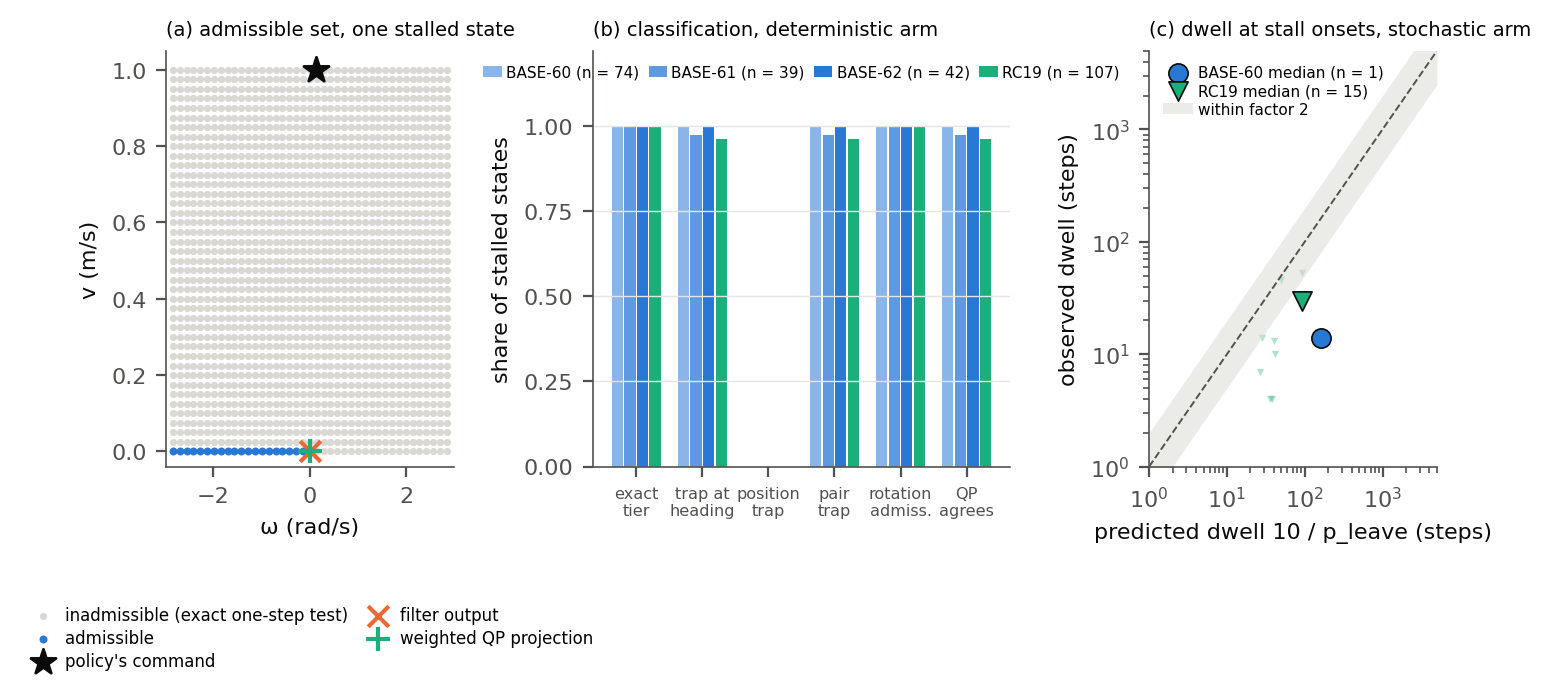
\includegraphics[width=\linewidth]{F6_geometry}
\caption{Stall geometry (round B1). (a)~The admissible set in $(v,\omega)$ at one archived stalled state, with the policy's command, the filter's output and the exact weighted projection. (b)~Classification of the stalled states of the deterministic arm per policy. (c)~Observed dwell beyond a stall onset in the stochastic arm against the geometric prediction, with the factor-two band.}
\label{fig:geometry}
\end{figure}

\begin{table}[t]
\centering\small
\caption{Round B1, deterministic arm: classification of stalled states (shares of $n$). Exact tier: the filter's exact tier handled the state. Trap at heading: no admissible command moves the body at the current heading. Position trap: no heading at the position admits motion. Rotation: an admissible rotation with $|\omega| \ge 0.5\,\wmax$ exists. QP: the exact weighted projection agrees with the filter's output. Law: the state arose on the intercept-law branch. Self-stop: share of immobile steps on which the nominal itself was zero.}
\label{tab:b1}
\begin{tabular}{@{}lrrrrrrrr@{}}
\toprule
Policy & $n$ & Exact tier & Trap at heading & Position trap & Rotation & QP agrees & Law & Self-stop \\
\midrule
BASE-60 & 74 & 1.00 & 1.00 & 0.00 & 1.00 & 1.00 & 1.00 & 0.41 \\
BASE-61 & 39 & 1.00 & 0.97 & 0.00 & 1.00 & 0.97 & 0.97 & 0.66 \\
BASE-62 & 42 & 1.00 & 1.00 & 0.00 & 1.00 & 1.00 & 1.00 & 0.57 \\
RC19 & 107 & 1.00 & 0.96 & 0.00 & 1.00 & 0.96 & 0.57 & 0.00 \\
\bottomrule
\end{tabular}
\end{table}

Round B1 measured Proposition~\ref{prop:stall} on four policies against the learned attacker, 100 episodes each with deterministic actions and the same 100 seeds with stochastic sampling (Figure~\ref{fig:geometry}, Table~\ref{tab:b1}). All 262 stalled states lie on the exact tier. Pooled over policies, 98.1\% are filter traps at the current heading and none is a position trap; an admissible rotation exists at every one of them. The exact weighted projection, computed by sequential least squares from four starts, agrees with the filter's output in 98.1\% of the states and yields forward motion in the remaining 1.9\%, which are exactly the five states that are not traps at heading. The registered bar for agreement was 99\%, so Proposition~\ref{prop:stall} is stated for the exact tier with this share: in 98\% of stalled states the stall is a property of the admissible set, and in 2\% it is a property of the filter's candidate enumeration. The registered dwell test failed. The deadlock rate under stochastic sampling is 0.42, 0.24, 0.29 and 0.57 against 0.38, 0.20, 0.21 and 0.55 with deterministic actions, so the loop survives exploration on four of four policies, but the geometric dwell prediction could not be tested on two policies, whose stochastic-arm stall onsets all occurred on the intercept-law branch, and over-predicted the observed median dwell by a factor of 3 to 12 on the other two. The intercept law produced 57 to 100\% of the stalled states; the same stall was observed in a rule-based pursuer in a separate game and is not a learning failure. Self-stops, the second kind of zero of (R4), are 41 to 66\% of the BASE policies' immobile steps and absent for RC19.

\subsection{Remedies}\label{sec:remedies}

\begin{figure}[t]
\centering
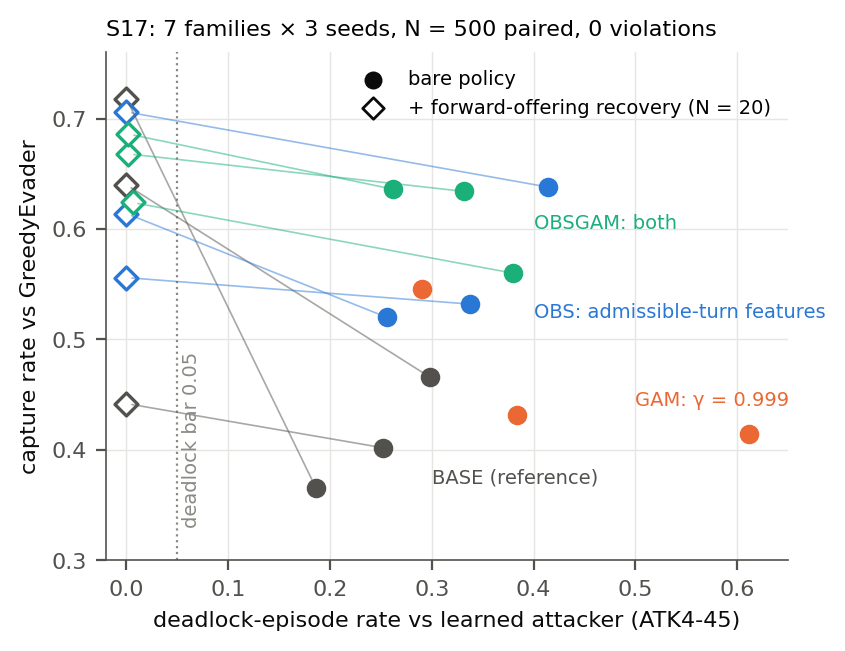
\includegraphics[width=\linewidth]{F3_remedies}
\caption{Round S17, 21 arms: deadlock-episode rate against the learned attacker versus capture rate against the greedy evader, $N = 500$ paired per cell. Hue marks the family, shape marks whether the recovery is present. The registered deadlock bar is 0.05.}
\label{fig:remedies}
\end{figure}

\begin{figure}[t]
\centering
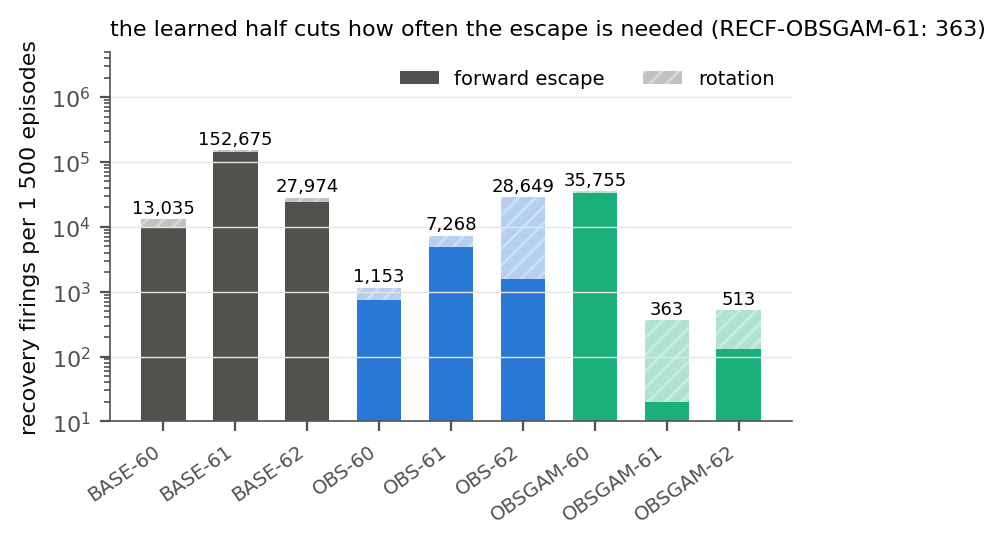
\includegraphics[width=\linewidth]{F4_firings}
\caption{Round S17: recovery firings per family over the 1\,500 gate episodes, split into forward and rotation candidates.}
\label{fig:firings}
\end{figure}

Round S16 trained five learning-side remedies from scratch, three seeds each, and added a scripted rotation-only recovery. Observation features and a longer horizon lowered immobility and raised capture without clearing the deadlock; the recurrent arm was confounded by an amendment to its batch settings and licenses no conclusion about memory; the stall penalty backfired (Section~\ref{sec:dissociations}). The rotation-only recovery scored 0.000 deadlock episodes in all nine cells and did so by spinning, with up to 277 firings per episode. Its anatomy showed that a straight command would have moved the body in every sampled stalled pose, which is the design rationale for offering forward candidates first.

Round S17 then compared seven families of three seeds each (Figures~\ref{fig:remedies} and~\ref{fig:firings}). Against the learned attacker the deadlock-episode rate of the BASE family is 0.298, 0.186 and 0.252; with the forward-offering recovery at $N = 20$ it is 0.000 on all three seeds, 0.000 on the three OBS seeds, and 0.006, 0.002 and 0.002 on the three OBSGAM seeds, against a registered bar of 0.05. Capture against the greedy evader rises significantly on nine of nine recovery seeds (BASE 0.466, 0.366, 0.402 to 0.640, 0.718, 0.442; $p \le 3.6\times10^{-5}$). The bare learned families raise capture too (OBS 0.532, 0.520, 0.638; GAM 0.546, 0.432, 0.414; OBSGAM 0.560, 0.634, 0.636) and leave the deadlock rate between 0.26 and 0.61. Every remedy that learns improves the task; only the escape removes the failure. The learned remedies change how often the recovery is needed: the RECF-BASE seeds fire 13\,035, 152\,675 and 27\,974 times over 1\,500 episodes, the RECF-OBSGAM seeds 35\,755, 363 and 513, a two-to-three-order reduction for equal capture. Zero contact steps occurred in about 31 million filtered gate steps. A registered anti-spin test passed on every arm and is uninformative, because the arm it was written to catch was not in the round.

\begin{figure}[t]
\centering
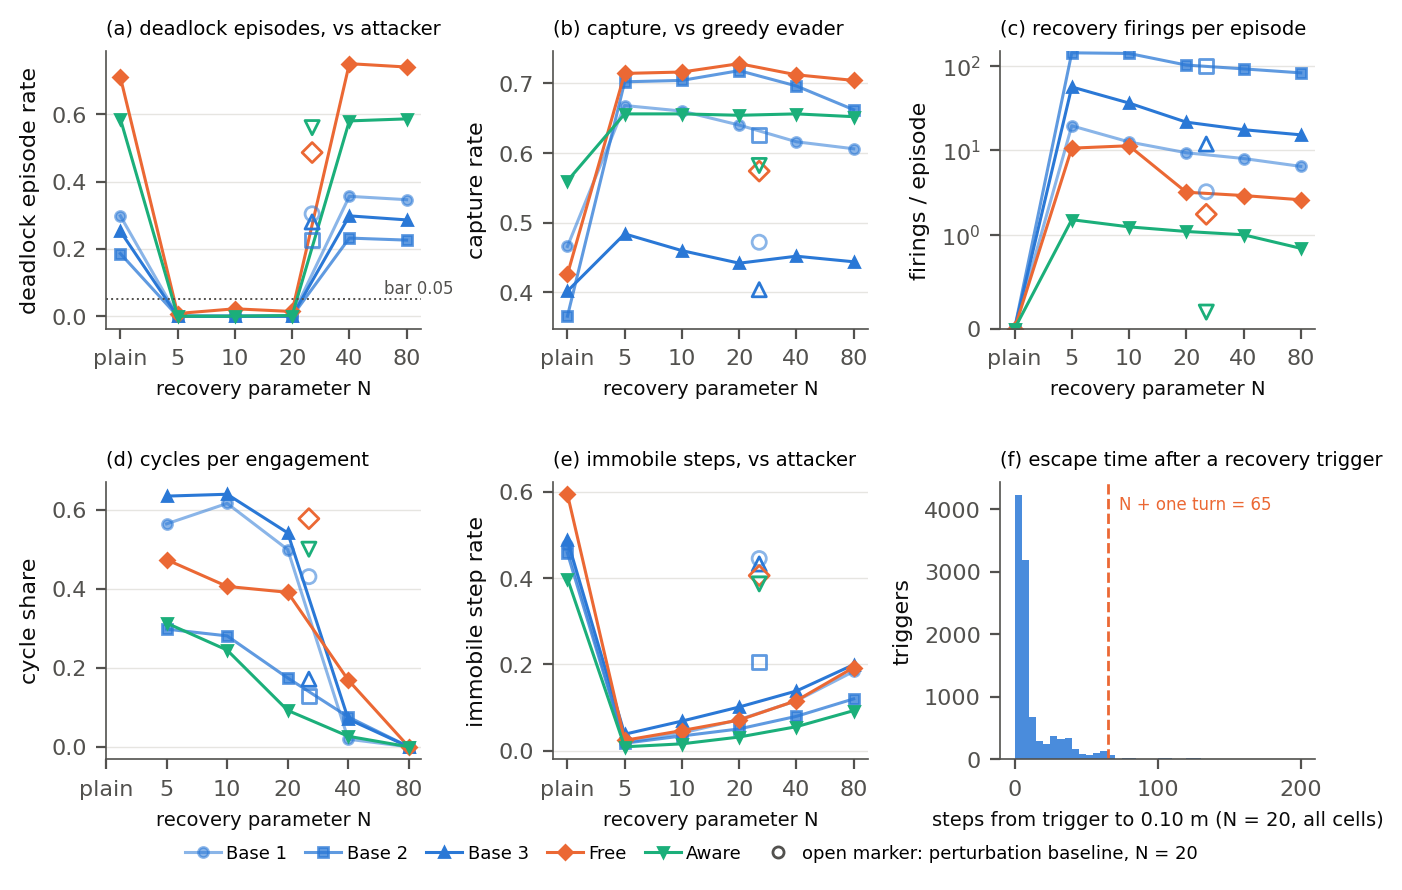
\includegraphics[width=\linewidth]{F7_recovery_sweep}
\caption{Round B2, five policies, $N = 500$ paired per cell. (a)~Deadlock-episode rate against the learned attacker and (b)~capture against the greedy evader as functions of the recovery parameter; open markers are the perturbation baseline at $N = 20$. (c)~Recovery firings per episode. (d)~Cycles per engagement. (e)~Immobile-step rate against the attacker. (f)~Steps from a trigger to a \SI{0.10}{m} displacement for $N = 20$, all cells, with the $N + T_{\mathrm{turn}}$ bound.}
\label{fig:sweep}
\end{figure}

Round B2 swept the recovery parameter over $N \in \{5,10,20,40,80\}$ on five policies, including the two from the rounds in which the failure was first seen, and added a perturbation baseline (Figure~\ref{fig:sweep}). Capture against the greedy evader is never significantly below the plain filter at any $N$ on any policy and is significantly above it at every $N$ on all five; the deadlock rate against the attacker is at most 0.022 for $N \le 20$ on all five (BASE 0.000; STR14 0.008, 0.022, 0.014; RC19 0.000, 0.000, 0.002), against 0.186 to 0.710 under the plain filter. For $N \ge 40$ the 40-step deadlock indicator is insensitive by construction, and the stall-run thresholds show the recovery working: runs of at least 80 steps are 0.000 to 0.020 of episodes at $N = 40$, and runs of at least 160 steps 0.000 to 0.016 at $N = 80$, against 0.176 to 0.682 under the plain filter. For the policies of the discovery, STR14's capture rises from 0.426 to 0.728 ($p = 7\times10^{-46}$) and its immobile-step rate against the attacker falls from 0.594 to 0.071; RC19's rise from 0.560 to 0.654 ($p = 10^{-14}$) and fall from 0.398 to 0.032.

The bound of Proposition~\ref{prop:recovery}(b) holds for 97.8\% of the 10\,475 decidable triggers at $N = 20$; eight of ten cells are above 98.5\%, and the two cells of one policy (BASE-62) are at 94.5 and 92.3\%, below the registered 95\% bar. The median escape takes 4 to 8 steps at every $N$. The cost of the recovery is cycles rather than immobility: at $N = 20$ the immobile-step rate is 0.023 to 0.101 on every cell, and between 0.08 and 0.56 of engagements are cycles, with the two policies that fire most (BASE-60 and BASE-62) near 0.5.

The perturbation baseline draws up to eight commands uniformly from the box after 20 immobile steps, filters each, and executes the first whose filtered speed exceeds $0.05\,\vmax$, the usual random resolution of a deadlock. It was registered with the expectation that it would also clear the deadlock and lose on capture and firings. It does not clear the deadlock on any of the five policies (0.304, 0.226, 0.280, 0.486, 0.560 against 0.298, 0.186, 0.252, 0.710, 0.586 plain). The recovery captures more than the baseline on five of five policies and fires more on five of five. The geometry of Figure~\ref{fig:geometry}(a) explains both: at a trap at heading the admissible set is the zero-speed segment, no sampled command moves, and a baseline that executes only moving commands can never rotate out, so its firings land on self-stops and never on the trap (one policy fires it 99 times per episode with its deadlock rate unchanged). Between 5 and 89\% of the recovery's firings at $N = 20$ are rotations. The recovery's contribution is the rotation candidate, not the trigger.

\subsection{A second filter}\label{sec:second}

\begin{figure}[t]
\centering
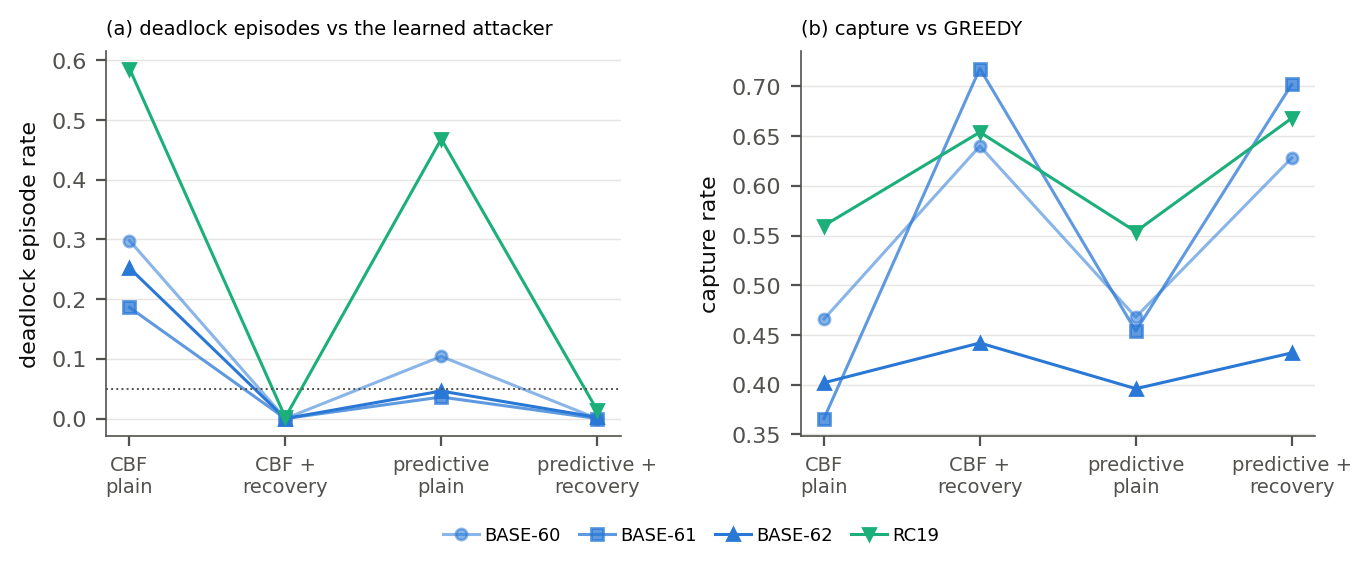
\includegraphics[width=0.9\linewidth]{F8_predictive}
\caption{Rounds B3 and B4, four policies, $N = 500$ paired: (a)~deadlock-episode rate against the learned attacker and (b)~capture against the greedy evader under the CBF filter and the predictive filter, each without and with the recovery at $N = 20$.}
\label{fig:predictive}
\end{figure}

Round B3 replaced the CBF projection with a sampling lookahead of horizon 4 through the simulator (Figure~\ref{fig:predictive}). The deadlock rate against the attacker is 0.104, 0.036, 0.046 and 0.468 on the four policies, against 0.298, 0.186, 0.252 and 0.586 under the CBF filter; paired, the CBF filter deadlocks more on seven of eight cells ($p \le 0.002$), and the exception is RC19 against the greedy evader, where the predictive filter deadlocks more (0.386 against 0.284). The registered bar, a rate of at least 0.05 on three of four policies, was met on two, so the loop is reported as present but weaker under the predictive filter at this lookahead. Round B4 composed the recovery onto the predictive filter by method resolution, so that every candidate is accepted or rejected by the predictive test; a construct gate re-filtered all 39\,162 commands of the first five episodes of each cell through a fresh predictive filter and found no rejection. The composition clears the deadlock (0.000, 0.000, 0.002, 0.014) and raises capture over the plain predictive filter on four of four policies (0.468 to 0.628, 0.454 to 0.702, 0.396 to 0.432, 0.554 to 0.668; all $p < 0.05$).

\section{Three dissociations: liveness metrics versus the task}\label{sec:dissociations}

\begin{figure}[t]
\centering
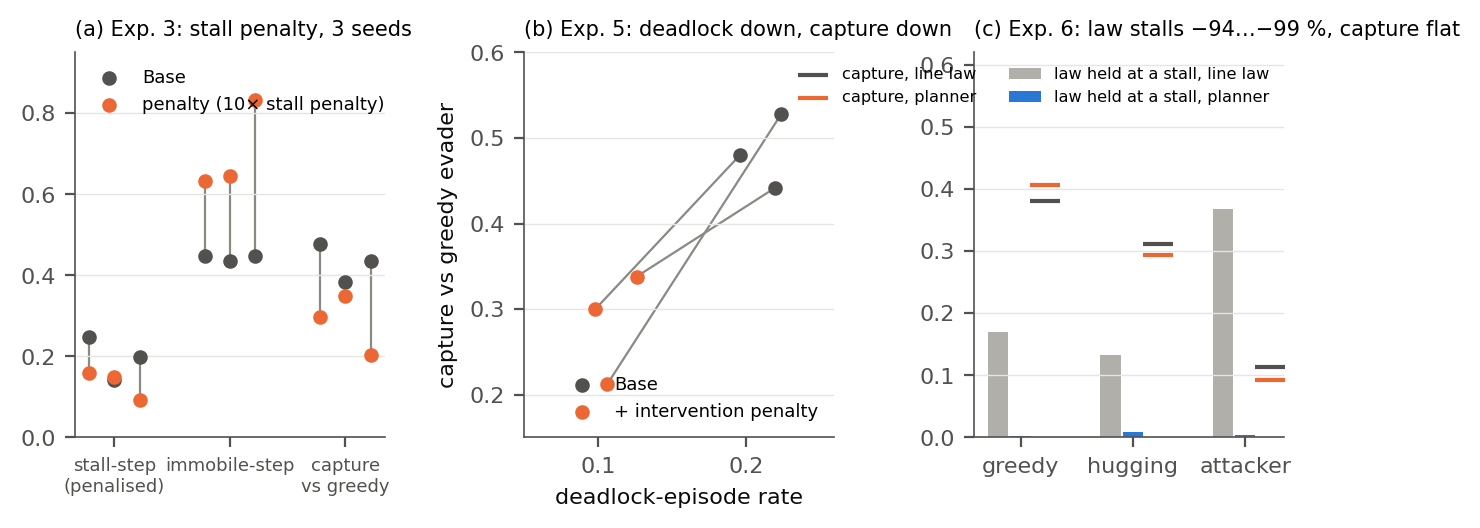
\includegraphics[width=\linewidth]{F5_dissociations}
\caption{Three pre-registered dissociations. (a)~Round S16: the stall penalty against its baseline, three seeds, stalled-step rate, immobile-step rate and capture. (b)~Round S18: the correction-magnitude penalty, deadlock-episode rate and capture, three seeds. (c)~Round S19: law-pinned episodes and capture for the line law and the planner law, three opponents.}
\label{fig:dissociations}
\end{figure}

Each of the following was a pre-registered hypothesis that failed in the registered direction (Figure~\ref{fig:dissociations}).

\paragraph{A stall penalty teaches the agent to stop asking.} In round S16 the PEN family, trained with a penalty on stalled steps, halves the stalled-step rate (0.143--0.249 to 0.093--0.158) while its immobile-step rate rises from 0.436--0.448 to 0.633--0.833 and its capture against the greedy evader falls from 0.384--0.478 to 0.204--0.348. The metric the penalty targets improves because the policy learns to emit a zero nominal, the second kind of zero of (R4); the fixed point is the same.

\paragraph{A correction-magnitude penalty improves the deadlock metric and hurts the task.} Round S18 trained 18 arms with the penalty of \citet{pizarro2025filtering} on the magnitude of the filter's correction; they square the correction and we use the unsquared norm in normalised action units, calibrated so that the expected episode penalty is one. In their quadrotor tracking task the penalty raised return and reduced chattering, and standing still is never a local optimum of a tracking reward. Here, in the dense-reward column, capture falls on three of three seeds (0.442, 0.480, 0.528 to 0.338, 0.300, 0.212; pooled $p = 3.6\times10^{-51}$) while zero-motion requests rise from 0.07, 0.16, 0.00 to 0.37, 0.78, 0.80, and the pre-registered deadlock metric improves in nine of nine cells (one seed from 0.224 to 0.106 while its immobile-step rate rises from 0.23 to 0.81). The penalty was charged for the intercept law's interventions as well as the head's, a confound that was registered and does not change the direction.

\paragraph{Removing the pins removes a symptom.} Round S19 replaced the intercept law with a planner that does not drive into obstacles. Episodes in which the law was held at a stall for at least 40 steps fall from 0.170, 0.132 and 0.368 to 0.002, 0.008 and 0.004 against the three opponents, a 94 to 99\% reduction, while filtered capture changes by $+0.026$, $-0.018$ and $-0.022$ ($p = 0.015$, $0.035$, $0.007$). The pins were a symptom; removing them left the task where it was.

\paragraph{Consequence.} A paper that evaluates a filtered learned policy should report the task, report immobility and stalled steps separately, and report firings per episode for any recovery it adds. A deadlock or intervention metric that improves under a penalty is a warning, not a result, until the task is shown to move with it.

\section{Discussion and limitations}\label{sec:discussion}

The claims are about memoryless policies. The one recurrent arm we trained was confounded before its number existed, so whether memory removes the failure is untested here, and we do not claim that it would. The environment is one game with one dynamics model and two filter constructions; the policies are trained from scratch for 5\,M steps or taken from 10\,M-step rounds; every family has three seeds and every cell 500 paired episodes. The discount argument of Remark~\ref{rem:discount} is a bound: the family with the longer horizon shows that the horizon is implicated and that lengthening it is not sufficient. The stalls of the scripted intercept law are the same fixed point as the learned head's and are not learning failures; Proposition~\ref{prop:stall} does not distinguish the two.

The recovery has a cost, and we measured rather than argued it away. Its stall--recover--stall cycles are between 8 and 56\% of engagements at $N = 20$, its escape bound fails on 2.2\% of triggers, and its firing count varies by three orders of magnitude across policies that capture equally well. The cheapest alternative, a random perturbation that accepts only moving commands, cannot leave a trap at heading at all. A perturbation that accepted rotations would be a different baseline, and we did not run it.

The process deserves one paragraph. Fifteen specifications passed their bars while measuring the artefact this paper is about, and the failure was found by a person watching the animated episodes, not by a registered test; the discovery episode showed 1\,085 consecutive blocked requests with a command standard deviation of 0.002, on an unregistered diagnostic of 100 episodes. Watching the behaviour has been part of our protocol since, as a construct gate that refuses to summarise a round before its designated episodes have been seen. We recommend it.

In practice: keep the filter, add the counter, log the firings, and watch the episodes.

\section{Conclusion}\label{sec:conclusion}

A minimal-intervention safety filter in front of a memoryless learned policy can create a closed-loop fixed point at which the guarantee holds, violations are zero, and the task fails silently. We characterised the fixed point, showed that its geometry is the admissible set's and not the learner's, measured why the learner cannot see the way out, and showed across seven pre-registered rounds that learning-side remedies improve the task without removing the failure while a one-counter recovery drawn from the same admissible set removes it with the guarantee untouched. Three dissociations show that the liveness metrics commonly reported next to a violation count can improve while the task collapses. The failure is cheap to remove and easy to miss; the second point is the one we would like this paper to change.

\paragraph{Reproducibility.} The environment, filters, policies, pre-registration documents, frozen commits, per-cell records and animated episodes for every round are released at [repository URL]. Each round's record names its commit and seed stream, and each figure's data file names its records.

\subsection*{Generative AI Use}

Generative AI tools were used for methodology drafting, coding and experimental implementation, literature search, and writing and editing. The authors reviewed and verified all AI-assisted content and take responsibility for the final content of the paper.

\bibliography{../references}

\end{document}
